% ==========================================
% BAB IV DESAIN KONSEP SOLUSI
% ==========================================
\setcounter{chapter}{3}  
\chapter{DESAIN KONSEP SOLUSI}
\label{chap:desain-konsep-solusi}

Bab ini berisi penjelasan secara rinci mengenai rancangan sistem yang diusulkan dalam 
penelitian ini, yaitu desain modul \textit{mission} dan \textit{exfiltration} pada \textit{spyware} dengan mode 
\textit{stealth} yang digunakan untuk menguji kapabilitas deteksi \textit{anti-spyware} dalam lingkungan terisolasi. 

\section{Tahapan Desain}
\label{sec:tahapan-desain}

\subsection{Rancangan Modul \textit{Mission}}
\label{subsec:rancangan-mission}

Rancangan modul \textit{Mission} disusun untuk mendefinisikan bagaimana proses pengambilan 
data (\textit{data crawling}) dijalankan secara tersembunyi (\textit{stealth}) pada sistem 
target. Modul ini berfungsi sebagai komponen utama yang menangani identifikasi artefak 
target, eksekusi proses \textit{crawling} secara terjadwal, serta pengendalian tingkat 
aktivitas agar tidak menimbulkan pola perilaku mencurigakan. Seluruh mekanisme di dalamnya 
dirancang dengan pendekatan \textit{fileless execution}, pengacakan interval, dan lapisan 
\textit{anti detection} untuk memastikan bahwa proses berjalan tanpa memicu peringatan 
dari mekanisme keamanan. Bagian ini mencakup arsitektur modul, jenis data yang menjadi target 
\textit{crawling}, lingkungan operasi, serta teknik-teknik \textit{crawling stealth} yang 
digunakan dalam pengembangan sistem.

\subsubsection{Arsitektur Modul \textit{Mission}}
\label{subsubsec:arsitektur-mission}

Modul \textit{mission} berfungsi sebagai inti proses \textit{crawling} data dalam sistem
\textit{spyware} mode \textit{stealth}, dengan tujuan utama melakukan pengumpulan informasi
secara diam-diam tanpa terdeteksi perangkat keamanan. Arsitektur modul ini
mengutamakan teknik \textit{fileless} dan \textit{evasion} agar proses kerja tidak
meninggalkan artefak digital di disk, serta meminimalisir kemungkinan identifikasi
oleh \textit{anti spyware}.

\begin{figure}[H]
    \centering
    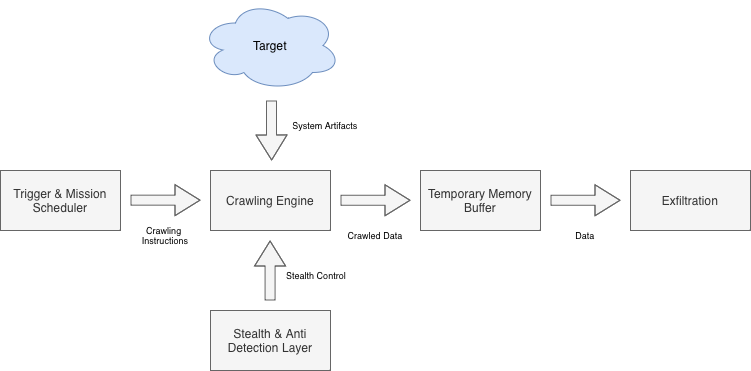
\includegraphics[width=0.95\textwidth]{image/arsitektur-mission.png}
    \caption{Diagram Blok Arsitektur Modul \textit{Mission}}
    \label{fig:arsitektur-mission}
\end{figure}

Secara umum, arsitektur modul \textit{Mission} yang akan dirancang terdiri dari empat 
komponen utama, yaitu:

\begin{enumerate}
    \item \textit{Trigger \& Mission Scheduler}

    \textit{Trigger \& mission scheduler} merupakan lapisan yang bertanggungjawab 
    memulai eksekusi misi berdasarkan interval waktu, kondisi sistem, atau pemicu 
    tertentu. \textit{Scheduler} memastikan bahwa proses \textit{crawling} tidak berjalan 
    secara terus-menerus, melainkan dieksekusi dalam \textit{batch} kecil dengan pola 
    waktu yang acak. Pendekatan ini bertujuan untuk menghindari karakteristik eksekusi 
    berulang dan berurutan, karena pola tersebut sering dianggap mencurigakan oleh 
    sistem deteksi berbasis perilaku.

    \item \textit{Data Crawling Engine}

    Komponen \textit{crawling engine} merupakan inti dari proses pengambilan data pada 
    sistem target. \textit{Engine} ini menangani tugas enumerasi artefak, pembacaan 
    \textit{file} atau metadata, serta pengambilan informasi sensitif lainnya yang relevan. 
    Proses \textit{crawling} dirancang agar bersifat modular sehingga dapat menyesuaikan 
    jenis artefak yang dituju. Seluruh proses berjalan dengan intensitas yang dikendalikan, 
    menggunakan API bawaan sistem dan teknik khusus seperti \textit{low-frequency access}, 
    sehingga aktivitas \textit{crawling} menyerupai perilaku rutin sistem operasi. Dengan 
    begitu, \textit{crawling engine} dapat mengakses data yang diperlukan tanpa 
    menimbulkan lonjakan I/O atau pola akses abnormal yang dapat memicu alarm 
    \textit{anti spyware}.

    \item \textit{Stealth \& Anti Detection Layer}

    Komponen \textit{stealth \& anti detection layer} berfungsi untuk menjaga agar 
    seluruh aktivitas modul \textit{Mission} tetap tersembunyi dari mekanisme 
    \textit{anti spyware}. Pada lapisan ini diimplementasikan \textit{anti VM}, 
    \textit{anti sandbox}, dan \textit{anti debugging} yang memungkinkan modul 
    mendeteksi lingkungan yang tidak aman dan menunda proses sampai kondisi normal. 
   Selain itu, lapisan ini mengontrol batasan intensitas \textit{crawling} melalui pengaturan 
   waktu jeda, pembatasan durasi eksekusi, serta pengacakan interval. Teknik 
   \textit{living-off-the-land} (LOTL) seperti pemanfaatan PowerShell, WMI, atau proses-proses 
   internal sistem juga digunakan untuk menyamarkan jejak eksekusi.

   \item \textit{Stealth \& Anti Detection Layer}
   
   \textit{Temporary memory buffer} merupakan ruang penyimpanan sementara yang menampung hasil 
   \textit{crawling} sebelum proses eksfiltrasi dilakukan. Sesuai dengan prinsip \textit{memory-resident} 
   pada \textit{fileless architecture}, \textit{buffer} ini diletakkan sepenuhnya di memori untuk menghindari 
   pembuatan artefak fisik pada disk yang dapat menjadi bukti forensik. Data yang terkumpul 
   disimpan dalam bentuk terstruktur dan dapat mengalami proses kompresi ringan agar lebih 
   efisien. \textit{Buffer} juga dilengkapi mekanisme penghapusan otomatis setelah sesi eksfiltrasi 
   selesai, sehingga tidak meninggalkan residu yang dapat dianalisis. \textit{Buffer} juga menjadi 
   indikator kesiapan eksfiltrasi karena proses pengiriman data hanya dilakukan ketika 
   kapasitas tertentu tercapai atau ketika misi menyelesaikan satu \textit{batch crawling}.

\end{enumerate}

Untuk mewujudkan arsitektur modul \textit{Mission}, diperlukan pemilihan teknologi
yang tepat agar setiap komponen dapat berfungsi sesuai karakteristiknya.
Arsitektur tersebut memerlukan mekanisme eksekusi yang ringan, fleksibel, serta
mampu berjalan sepenuhnya secara \textit{fileless} tanpa meninggalkan jejak digital
pada \textit{disk}. Selain itu, modul \textit{Mission} harus mendukung teknik 
\textit{living-off-the-land}, implementasi \textit{anti analysis}, serta pengelolaan data 
\textit{in memory} agar aktivitas \textit{crawling} dapat berlangsung secara \textit{stealth} 
dan tidak memicu sistem deteksi \textit{anti spyware}. Oleh karena itu, teknologi yang 
digunakan harus mampu mengakomodasi operasi \textit{low level} pada sistem, menyediakan 
akses ke artefak sistem, serta sekaligus mendukung eksekusi yang tersamarkan. 
Pada Tabel \ref{tbl:teknologi-mission} dibahas teknologi yang digunakan untuk 
mengimplementasikan setiap komponen modul \textit{Mission} serta alasan pemilihannya.

\begin{table}[H]
\centering
\captionsetup{justification=raggedright,singlelinecheck=false}
\caption{Teknologi yang Digunakan pada Setiap Komponen Modul \textit{Mission}}
\label{tbl:teknologi-mission}

\renewcommand{\arraystretch}{1.4}
\begin{tabular}{|p{5cm}|p{8cm}|}
\hline
\textbf{Komponen Modul Mission} & \textbf{Teknologi yang Digunakan} \\
\hline

\textit{Trigger \& Mission Scheduler} &
\begin{itemize}[leftmargin=1.2em]
    \item Python (\texttt{time}, \texttt{random}, \texttt{asyncio})
    \item Jitter-based interval scheduling
\end{itemize}
\\
\hline

\textit{Data Crawling Engine} &
\begin{itemize}[leftmargin=1.2em]
    \item Python (\texttt{os}, \texttt{pathlib}, \texttt{psutil}, \texttt{subprocess})
    \item PowerShell
    \item WMI
    \item Win32 API
\end{itemize}
\\
\hline

\textit{Stealth \& Anti Detection Layer} &
\begin{itemize}[leftmargin=1.2em]
    \item Win32 API
    \item PowerShell
    \item LOLBins
\end{itemize}
\\
\hline

\textit{Temporary Memory Buffer} &
\begin{itemize}[leftmargin=1.2em]
    \item Python (\texttt{io.BytesIO}, \texttt{zlib})
\end{itemize}
\\
\hline

\end{tabular}
\end{table}


\subsubsection{Target Data dan Lingkungan Operasi}
\label{subsubsec:target-data-lingkungan-operasi}

Modul \textit{Mission} dirancang untuk mengumpulkan data yang relevan dengan 
pemetaan aktivitas sistem dan pengguna, serta mendukung proses analitik pada 
tahap selanjutnya. Data yang dikumpulkan berfokus pada artefak yang dapat 
memberikan gambaran mengenai perilaku sistem tanpa mengambil konten sensitif 
secara langsung. Secara garis besar, terdapat X kelompok utama data yang 
menjadi target \textit{crawling}.

\begin{table}[h]
\captionsetup{justification=raggedright,singlelinecheck=false}
\centering
\begin{tabular}{ | p{3cm} | p{4.5cm} | p{4cm} | p{2cm} | }
    \hline
    \textbf{Kategori Data} & \textbf{Deskripsi} 
    & \textbf{Atribut Utama} & \textbf{Contoh Nilai} \\ 
    \hline

    Hasil \textit{Keylogging} &
    Rekaman aktivitas penekanan tombol secara kronologis. &
    timestamp, key\_code, process\_name &
    -- \\
    \hline

    Metadata Proses Sistem &
    Informasi konteks eksekusi proses pada saat aktivitas terjadi. &
    pid, process\_name, cpu\_usage, memory\_usage, start\_time, end\_time &
    -- \\
    \hline

    Artefak Sistem Tambahan &
    Artefak yang menggambarkan kondisi sistem saat \textit{crawling}. &
    active\_window, running\_processes, focus\_change &
    -- \\
    \hline
\end{tabular}
\caption{Tabel IV.2 Target Data}
\label{tbl:target-data}
\end{table}


Seluruh proses \textit{crawling} pada modul \textit{Mission} dijalankan di 
dalam lingkungan terisolasi menggunakan \textit{Virtual Machine (VM)} berbasis 
Windows 10/11 (64-bit). Penggunaan \textit{VM} dipilih untuk memastikan bahwa 
pengujian berlangsung secara aman, tidak memengaruhi sistem utama, serta 
memungkinkan proses \textit{rollback} melalui \textit{snapshot} apabila terjadi 
kesalahan selama eksperimen. Modul berjalan pada level pengguna 
(\textit{user-level access}) tanpa hak administratif, sehingga mencerminkan 
kondisi bagaimana \textit{spyware} berbasis \textit{stealth} beroperasi. Selain 
itu, proses \textit{crawling} hanya dilakukan apabila kondisi lingkungan dinilai 
aman untuk menjaga karakteristik \textit{stealth} dari modul yang dirancang.

\subsubsection{Alur Kerja Modul \textit{Mission}}
\label{subsubsec:alur-kerja-mission}

Alur kerja modul \textit{Mission} menggambarkan urutan proses yang dijalankan 
selama tahap pengumpulan data berlangsung, mulai dari pemicu eksekusi, pemeriksaan 
kondisi lingkungan, hingga penyimpanan data sementara dan persiapan eksfiltrasi. 
Secara keseluruhan, \textit{workflow} dirancang agar proses \textit{crawling} berjalan 
secara adaptif, terkontrol, dan tetap mempertahankan karakteristik \textit{stealth} agar 
tidak terdeteksi oleh mekanisme pertahanan sistem. Diagram alur pada Gambar 
\ref{fig:flowchart-mission} memperlihatkan langkah-langkah utama yang dilakukan oleh 
modul ini.

\begin{figure}[H]
    \centering
    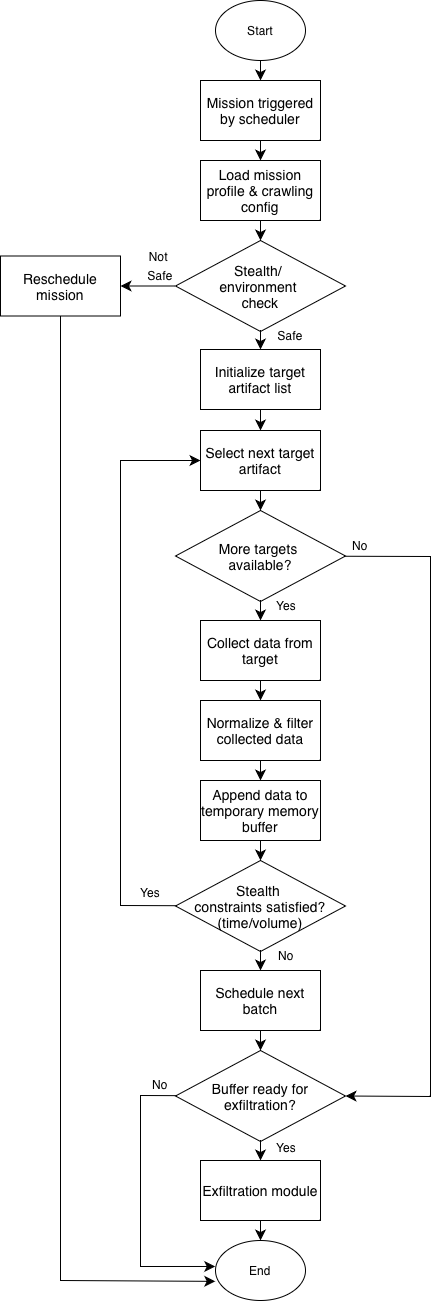
\includegraphics[width=0.45\textwidth]{image/flowchart-mission.png}
    \caption{\textit{Flowchart} Alur Kerja Modul \textit{Mission}}
    \label{fig:flowchart-mission}
\end{figure}

Proses dimulai ketika \textit{Mission Scheduler} memicu eksekusi modul sesuai interval 
waktu yang telah diacak untuk menghindari pola statis. Setelah modul mulai berjalan, 
konfigurasi misi dan profil \textit{crawling} dimuat ke dalam memori untuk menentukan 
jenis data yang harus dikumpulkan pada \textit{batch} eksekusi tersebut. Sebelum proses 
\textit{crawling} dilakukan, modul menjalankan \textit{stealth/environment check} untuk 
memastikan bahwa kondisi perangkat aman. Pada tahap ini, sistem memeriksa indikasi 
keberadaan \textit{sandbox, debugger,} atau aktivitas sistem yang tidak wajar. Jika 
lingkungan dianggap tidak aman, misi tidak dilanjutkan dan dijadwalkan ulang pada waktu 
berikutnya.

Apabila kondisi aman, modul \textit{Mission} menginisialisasi daftar artefak target yang 
akan diproses, seperti metadata proses aktif atau \textit{buffer keylogging} yang perlu 
dipindai. Modul kemudian memilih target berikutnya dari daftar, dan memeriksa apakah masih 
terdapat artefak yang harus dikumpulkan. Jika tidak ada target tersisa, \textit{batch crawling} 
dianggap selesai dan proses dapat berlanjut ke tahap berikutnya.

Untuk setiap target yang tersedia, modul mengambil data melalui \textit{crawling engine}. 
Proses ini mencakup pembacaan metadata sistem maupun pengambilan \textit{buffer} hasil 
penekanan tombol. Data mentah yang diperoleh kemudian dinormalisasi, difilter, dan disesuaikan 
dengan format penyimpanan sementara agar tetap efisien dan konsisten. Setelah diproses, data 
ditambahkan ke dalam \textit{temporary memory buffer} yang berada sepenuhnya di memori untuk 
menjaga sifat \textit{fileless}.

Selanjutnya, modul melakukan evaluasi terhadap batasan \textit{stealth}, seperti durasi eksekusi 
maksimum atau volume data per \textit{batch}. Jika batasan belum terpenuhi, modul menjadwalkan 
\textit{batch crawling} berikutnya dan kembali ke proses pemilihan target. Jika batasan terpenuhi, 
modul bergerak ke tahap selanjutnya, yaitu memeriksa apakah \textit{buffer} siap untuk 
dieksfiltrasi. Pemeriksaan ini dapat berbasis ukuran \textit{buffer}, jumlah entri yang terkumpul, 
atau kondisi khusus lainnya.

Jika \textit{buffer} belum memenuhi kriteria eksfiltrasi, modul kembali ke proses \textit{crawling} 
pada \textit{batch} berikutnya. Namun, apabila \textit{buffer} telah mencapai kondisi siap kirim, 
modul \textit{Mission} mengaktifkan komponen eksfiltrasi dan menyerahkan data untuk dikirim ke modul 
berikutnya. Setelah proses eksfiltrasi selesai, eksekusi modul \textit{Mission} pada \textit{batch} 
tersebut diakhiri.

Dengan alur kerja ini, modul \textit{Mission} dapat melakukan pengumpulan data secara bertahap, 
efisien, dan tetap mempertahankan sifat \textit{stealth}. Pendekatan berbasis \textit{batch}, 
validasi lingkungan, dan kontrol frekuensi eksekusi memastikan proses berjalan tanpa memicu sistem 
deteksi maupun meninggalkan artefak yang dapat dianalisis.

\subsection{Rancangan Modul \textit{Exfiltration}}
\label{subsec:rancangan-exfiltration}

Rancangan modul \textit{Exfiltration} disusun untuk mendefinisikan bagaimana data hasil 
\textit{crawling} diproses, dikemas, dan dikirimkan ke \textit{endpoint} secara aman serta 
tetap mempertahankan karakteristik \textit{stealth}. Modul ini berfungsi mengelola 
penjadwalan pengiriman, menyiapkan \textit{payload} yang telah terstruktur, serta 
memastikan proses transmisi berlangsung tanpa memicu deteksi dari sistem keamanan. 
Mekanisme di dalamnya mencakup proses \textit{packaging, encoding, compression,} pemilihan 
waktu dan metode pengiriman, serta kontrol lingkungan sebelum data dikirim. Bagian ini membahas 
arsitektur modul eksfiltrasi, jenis \textit{output} yang dihasilkan, serta alur mekanisme 
pengiriman data dari \textit{buffer} hingga diterima oleh \textit{endpoint} analitik.

\subsubsection{Arsitektur Modul \textit{Exfiltration}}
\label{subsubsec:arsitektur-exfiltration}

Modul \textit{Exfiltration} bertanggungjawab untuk mengirimkan data hasil \textit{crawling} dari 
modul \textit{Mission} ke penerima dalam bentuk yang terstruktur, aman, dan tetap mempertahankan 
sifat \textit{stealth}. Modul \textit{Exfiltration} berperan sebagai jembatan antara lingkungan 
eksekusi \textit{spyware} dan \textit{big data analytic}. Arsitektur modul ini dirancang agar 
dapat bekerja secara \textit{fileless}, meminimalkan jejak pada \textit{disk}, serta menggunakan 
pola pengiriman \textit{low and slow} sehingga tidak memicu deteksi anomali jaringan. 

\begin{figure}[H]
    \centering
    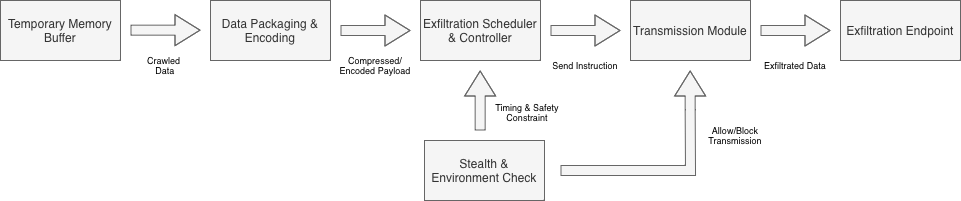
\includegraphics[width=0.95\textwidth]{image/arsitektur-exfiltration.png}
    \caption{Diagram Blok Arsitektur Modul \textit{Exfiltration}}
    \label{fig:arsitektur-exfiltration}
\end{figure}

Secara garis besar, arsitektur modul \textit{Exfiltration} terdiri dari beberapa komponen utama, yaitu: 

\begin{enumerate}
    \item \textit{Temporary Memory Buffer}

    \textit{Temporary memory buffer} berfungsi sebagai titik masuk (\textit{entry point}) bagi 
    modul \textit{Exfiltration}. \textit{Buffer} ini berisi kumpulan data hasil \textit{crawling} 
    modul \textit{Mission} yang disimpan sepenuhnya di memori. Dengan menempatkan 
    \textit{buffer} di RAM, arsitektur ini menghindari pembuatan \textit{file log} permanen 
    pada \textit{disk} sehingga konsisten dengan pendekatan \textit{fileless}. Modul 
    \textit{Exfiltration} tidak berinteraksi langsung dengan modul \textit{Mission}, melainkan 
    hanya membaca data yang sudah siap dari \textit{buffer} tersebut.

    \item \textit{Data Packaging \& Encoding}
    
    \textit{Data packaging \& encoding} bertugas mengubah data mentah dalam \textit{buffer} 
    menjadi payload yang siap dikirim. Pada tahap ini dilakukan proses normalisasi, 
    penggabungan, kompresi, serta encoding data. Tujuannya adalah mengurangi ukuran \textit{payload}, 
    menyamakan format antar \textit{batch}, dan mempermudah proses pengiriman melalui protokol 
    jaringan yang digunakan. Dengan demikian, data yang dikirim ke \textit{endpoint} bersifat 
    ringkas, konsisten, dan tidak mudah dikenali sebagai \textit{traffic} yang tidak biasa.

    \item \textit{Exfiltration Scheduler \& Controller}
    
    Komponen \textit{exfiltration scheduler \& controller} berperan sebagai pengatur waktu dan 
    ritme pengiriman. Modul ini menentukan kapan proses eksfiltrasi dijalankan, seberapa besar ukuran 
    \textit{batch} yang dikirim, serta mengatur interval pengiriman agar tidak menimbulkan lonjakan 
    lalu lintas jaringan. Pendekatan \textit{low frequency transmission} dan \textit{randomized interval} 
    diterapkan juga diterapkan sehingga pola pengiriman tidak tampak statis atau berulang. 
    \textit{Scheduler} juga mengelola status antrian pengiriman, misalnya menandai \textit{payload} 
    yang telah berhasil dikirim maupun yang perlu diulang.
    
    \item \textit{Stealth \& Environment Check}
    
    Komponen \textit{stealth \& environment check} yang memonitor kondisi lingkungan sebelum dan 
    selama proses eksfiltrasi. Komponen ini melakukan pengecekan terhadap indikator tertentu, seperti 
    beban CPU, ketersediaan jaringan, maupun adanya tanda-tanda lingkungan analisis (\textit{sandbox, debugger,} 
    atau \textit{monitoring} intensif). Hasil pengecekan ini digunakan sebagai \textit{constraint} 
    bagi \textit{exfiltration scheduler \& controller} dan \textit{transmission module}. Jika kondisi 
    tidak memenuhi kriteria \textit{stealth}, modul dapat menunda pengiriman, memperpanjang interval, 
    atau membatalkan proses eksfiltrasi untuk \textit{batch} tersebut.

    \item \textit{Transmission Module}
    
    Komponen \textit{transmission module} merupakan bagian yang melakukan pengiriman data 
    secara nyata ke pihak penerima. Modul ini mengolah \textit{payload} yang sudah dikemas 
    dan apabila sudah diizinkan oleh \textit{stealth layer} mengirimkannya melalui saluran 
    komunikasi yang telah ditentukan. \textit{Transmission module} didesain agar menyerupai 
    trafik aplikasi biasa, sehingga tidak mudah dibedakan dari aktivitas jaringan normal 
    oleh mekanisme pemantauan. 
    
    \item \textit{Exfiltration Endpoint}
    
    \textit{Exfiltration endpoint} merupakan komponen di sisi penerima yang menerima 
    \textit{payload} dari modul \textit{exfiltration}. \textit{Endpoint} ini berupa server 
    penerima di lingkungan terkontrol yang kemudian akan meneruskan data tersebut ke sistem 
    penyimpanan yang akan diolah dalam \textit{big data analytic}. 

\end{enumerate}

\subsubsection{Target Output \textit{Exfiltration}}
\label{subsubsec:target-output-exfiltration}

\textit{Output} eksfiltrasi merupakan data akhir yang telah dikumpulkan oleh modul 
\textit{Mission} dan diproses sebelum dikirimkan ke \textit{endpoint} tujuan. Secara umum, 
output yang dieksfiltrasi terdiri dari tiga kategori utama yang disajikan pada 
Tabel~\ref{tbl:target-output-exfiltration}.

\begin{table}[H]
\captionsetup{justification=raggedright,singlelinecheck=false}
\centering
\renewcommand{\arraystretch}{1.35}
\begin{tabular}{|p{5cm}|p{8cm}|}
\hline
\textbf{Komponen Modul \textit{Exfiltration}} & \textbf{Teknologi yang Digunakan} \\
\hline

\textit{Temporary Memory Buffer} &
\begin{itemize}[leftmargin=*]
    \item Python (\texttt{io.BytesIO}, \texttt{zlib})
\end{itemize}
\\
\hline

\textit{Data Packaging \& Encoding} &
\begin{itemize}[leftmargin=*]
    \item Python (\texttt{zlib}, \texttt{base64})
\end{itemize}
\\
\hline

\textit{Exfiltration Scheduler \& Controller} &
\begin{itemize}[leftmargin=*]
    \item Python (\texttt{time}, \texttt{random}, \texttt{asyncio})
    \item Jitter-based interval scheduling
    \item In-memory queue
\end{itemize}
\\
\hline

\textit{Stealth \& Environment Check} &
\begin{itemize}[leftmargin=*]
    \item Python (\texttt{psutil})
    \item Win32 API
\end{itemize}
\\
\hline

\textit{Transmission Module} &
\begin{itemize}[leftmargin=*]
    \item Python \texttt{requests} (HTTPS)
    \item Python (\texttt{ssl})
    \item PowerShell \texttt{Invoke-WebRequest} (LOLBins)
\end{itemize}
\\
\hline

\textit{Exfiltration Endpoint} &
\begin{itemize}[leftmargin=*]
    \item REST API (FastAPI)
\end{itemize}
\\
\hline

\end{tabular}
\caption{Teknologi yang Digunakan pada Modul \textit{Exfiltration}}
\label{tbl:teknologi-modul-exfiltration}
\end{table}


Sebelum dikirimkan, seluruh data dikemas dalam struktur \textit{payload} yang sudah
dikompresi dan di-\textit{encode}. \textit{Payload} dapat berupa JSON terstruktur sebelum
diberikan proses kompresi. Struktur \textit{payload} dipaparkan pada Tabel~\ref{tbl:struktur-payload}.

\begin{table}[H]
\captionsetup{justification=raggedright,singlelinecheck=false}
\caption{Target \textit{Output Exfiltration}}
\label{tbl:target-eksfiltrasi}

\raggedright
\begin{tabular}{|p{5cm}|p{7.9cm}|}
\hline
\textbf{Kategori Data} & \textbf{Deskripsi} \\
\hline

Hasil \textit{Keylogging} &
Rekaman aktivitas penekanan tombol secara kronologis. \\
\hline

Metadata Proses Sistem &
Informasi konteks eksekusi proses pada saat aktivitas terjadi. \\
\hline

Artefak Sistem Tambahan &
Artefak yang menggambarkan kondisi sistem saat \textit{crawling}. \\
\hline

Aktivitas \textit{cache internet browsing} &
Riwayat dan jejak akses halaman web yang tersimpan oleh browser. \\
\hline
\end{tabular}
\end{table}


\subsubsection{Mekanisme Pengiriman Data}
\label{subsubsec:mekanisme-pengiriman-data}

Mekanisme pengiriman data pada modul \textit{Exfiltration} dirancang untuk 
memastikan proses transfer berjalan secara aman, terkontrol, dan tidak 
menimbulkan pola komunikasi yang mudah dikenali oleh sistem pertahanan. 
Alur kerja ini digambarkan melalui diagram alur pada Gambar~\ref{fig:flowchart-exfiltration}, 
dimulai dari pemeriksaan kesiapan \textit{buffer}, penjadwalan waktu pengiriman, 
hingga proses pembersihan \textit{buffer} setelah data berhasil dikirimkan.

\begin{figure}[H]
    \centering
    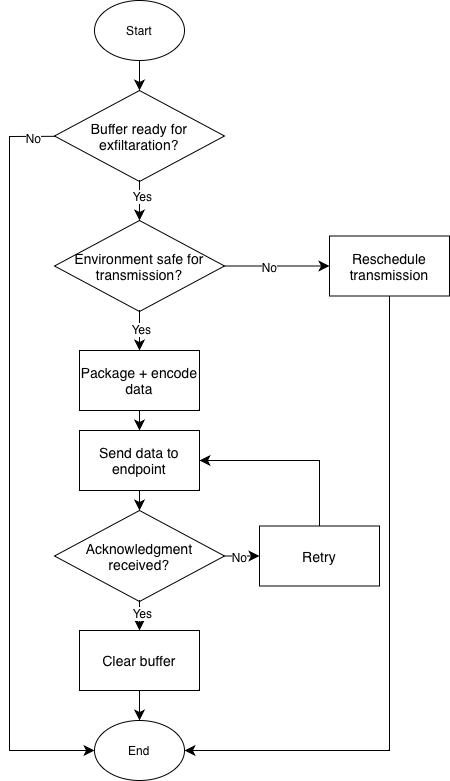
\includegraphics[width=0.60\textwidth]{image/flowchart-exfiltration.png}
    \caption{\textit{Flowchart} Mekanisme Pengiriman Data pada Modul \textit{Exfiltration}}
    \label{fig:flowchart-exfiltration}
\end{figure}

Proses dimulai dengan memeriksa apakah \textit{temporary memory buffer} 
telah mencapai kondisi siap untuk dikirim, baik berdasarkan ukuran muatan 
(\textit{payload size threshold}) maupun batas waktu 
(\textit{time threshold}). Jika \textit{buffer} belum siap, 
\textit{batch} dihentikan dan modul menunggu siklus berikutnya yang dipicu 
kembali oleh \textit{scheduler}. 

Apabila \textit{buffer} berada dalam kondisi siap, modul akan melakukan 
evaluasi lingkungan. Tahap ini memastikan bahwa sistem target berada dalam 
keadaan aman untuk melakukan komunikasi keluar. Jika kondisi dinilai tidak 
aman, modul tidak memaksakan pengiriman dan akan menjadwalkan ulang 
transmisi pada interval berikutnya.

Jika lingkungan aman, sistem memasuki tahap 
\textit{data packaging \& encoding}. Pada tahap ini, data hasil 
\textit{crawling} yang tersimpan di memori dikompresi dan di-\textit{encode} 
menggunakan teknik ringan agar ukuran paket lebih kecil dan pola data lebih 
sulit dianalisis. \textit{Payload} yang sudah dipaketkan kemudian dikirimkan 
ke \textit{endpoint} tujuan melalui modul transmisi.

Setelah pengiriman dilakukan, modul akan menunggu respons berupa 
\textit{acknowledgment} dari \textit{endpoint}. Jika 
\textit{acknowledgment} tidak diterima, modul akan mencoba melakukan 
\textit{retry} pengiriman sejumlah batas maksimum yang telah ditentukan. 
Proses \textit{retry} tetap berada dalam \textit{batch} yang sama. Jika 
seluruh percobaan gagal, modul akan mengakhiri \textit{batch} tanpa 
menghapus \textit{buffer} sehingga data tetap aman dan akan dicoba kembali 
pada siklus berikutnya.

Apabila \textit{acknowledgment} diterima, \textit{buffer} dianggap telah 
berhasil dieksfiltrasi. Modul kemudian melakukan \textit{buffer clearing} 
untuk menghapus seluruh data yang telah dikirim dari memori, sesuai dengan 
prinsip \textit{memory resident operation} pada arsitektur \textit{fileless}. 
Tahap ini sekaligus menandai berakhirnya satu siklus eksfiltrasi, dan modul 
kembali menunggu pemicu berikutnya dari \textit{scheduler}.

\subsubsection{Rancangan Lingkungan Pengujian}
\label{subsubsec:lingkungan-pengujian}

Lingkungan pengujian dirancang agar proses eksekusi modul 
\textit{Mission} dan \textit{Exfiltration} dapat dilakukan secara aman 
dan terkontrol. Seluruh percobaan dilakukan pada lingkungan Windows yang 
dikonfigurasi secara terisolasi sehingga aktivitas \textit{crawling} 
dan eksfiltrasi tidak berdampak pada sistem di luar area pengujian. 
Lingkungan uji yang digunakan disajikan pada Tabel~\ref{tbl:konfigurasi-pengujian}.

\begin{table}[H]
    \centering
    \captionsetup{justification=raggedright,singlelinecheck=false}
    \begin{tabular}{ | p{4cm} | p{9cm} | }
        \hline
        \textbf{\textit{Field}} & \textbf{Isi/Struktur} \\
        \hline
        keylogs & List objek \textit{keylogging} \\ 
        \hline
        process\_metadata & List metadata proses \\ 
        \hline
        system\_artifacts & Data artefak sistem \\ 
        \hline
        cache\_activity & List aktivitas \textit{cache/browsing} \\ 
        \hline
        session\_id & ID unik \textit{batch crawling} \\ 
        \hline
        generated\_at & \textit{Timestamp} waktu payload dibuat \\ 
        \hline
    \end{tabular}
    \caption{Struktur \textit{Payload}}
    \label{tbl:struktur-payload}
\end{table}

Lingkungan pengujian pada penelitian ini dibangun menggunakan sistem operasi Windows 
10/11 yang dikonfigurasi secara terisolasi untuk memastikan bahwa proses \textit{crawling} 
dan \textit{eksfiltrasi} tidak berdampak pada sistem di luar area eksperimen. Seluruh modul 
dijalankan menggunakan Python 3.x dan PowerShell sebagai bahasa pemrograman utama, dengan 
dukungan beberapa \textit{library} seperti \textit{psutil}, \textit{pathlib}, \textit{requests}, 
dan Win32API untuk mengakses artefak sistem serta mengelola proses \textit{crawling}. 
Proses \textit{exfiltration} diarahkan menuju sebuah \textit{endpoint} lokal berbasis 
\textit{REST API} (FastAPI) yang berfungsi sebagai server penerima \textit{payload} 
hasil \textit{crawling}. Konfigurasi ini memastikan bahwa seluruh aktivitas uji dapat 
dilakukan secara aman, terkontrol, dan sesuai dengan prinsip penelitian 
\textit{spyware mode stealth}.

\section{Hasil Desain}
\label{sec:hasil-desain}

Bagian ini merupakan hasil desain dari arsitektur sistem yang mencakup 
keseluruhan proses \textit{mission crawling} hingga \textit{data exfiltration}, yang 
menjadi fokus utama pada penelitian ini. Desain ini disusun untuk menunjukkan 
bagaimana modul-modul yang dibangun berinteraksi, bagaimana data bergerak dari 
sumber hingga tujuan akhir, serta bagaimana prinsip \textit{stealth} dipertahankan 
sepanjang alur eksekusi.

\begin{figure}[H]
    \centering
    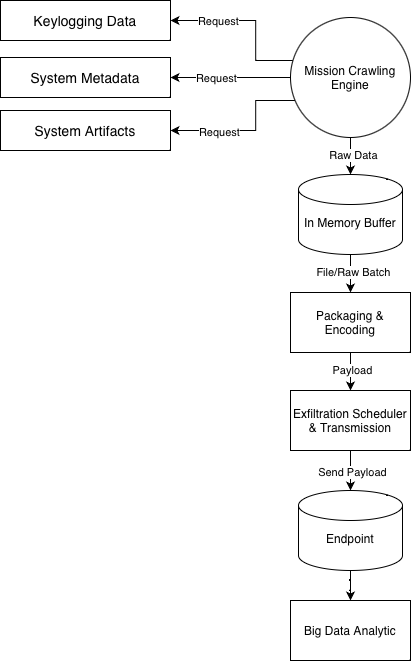
\includegraphics[width=0.45\textwidth]{image/hasil-desain.png}
    \caption{Diagram Hasil Desain Arsitektur Sistem}
    \label{fig:hasil-desain}
\end{figure}

Pada desain ini, sistem memulai proses dengan tiga kelompok data utama, yaitu 
\textit{keylogging data}, \textit{system metadata}, dan \textit{system artifacts}. 
Ketiganya diakses oleh \textit{Mission Crawling Engine} secara terjadwal melalui 
mekanisme \textit{request based crawling}. \textit{Engine} kemudian menghasilkan 
\textit{raw data} yang disimpan di \textit{In Memory Buffer}, yaitu ruang penyimpanan 
sementara yang bersifat \textit{memory resident} untuk menghindari terbentuknya jejak 
digital pada \textit{disk}.

Selanjutnya, data dari \textit{buffer} diproses dalam tahap \textit{Packaging \& Encoding}, 
di mana data dikemas, di-\textit{encode}, dan dikompresi menjadi sebuah \textit{payload} 
terstruktur. \textit{Payload} ini kemudian dikirim melalui 
\textit{Exfiltration Scheduler \& Transmission Module}, yang bekerja dengan memperhatikan 
batasan \textit{stealth} seperti pengacakan waktu pengiriman, pemilihan metode transmisi 
yang rendah anomali, serta mekanisme \textit{retry} bila konfirmasi tidak diterima. Data 
yang berhasil dieksfiltrasi akan tersimpan dalam \textit{Endpoint}, dan selanjutnya 
menjadi input bagi \textit{Big Data Analytic} untuk proses analisis lebih lanjut.